
\documentclass[12pt]{article}
\usepackage{geometry} % see geometry.pdf on how to lay out the page. There's lots.
\geometry{a4paper} % or letter or a5paper or ... etc
% \geometry{landscape} % rotated page geometry
\usepackage{color}
\usepackage{apacite}
\usepackage{graphicx}
\usepackage{subcaption}
\usepackage{float}
\usepackage[justification=centering]{caption}


% See the ``Article customise'' template for some common customisations

%%% BEGIN DOCUMENT
\begin{document}

%Title page
\noindent
Freie Universitat Berlin\\
FB Informatics / Mathematics\\
Cognitive Systems Seminar\\
Winter Term 2018/19\\
Instructor: Ana-Maria Olteteanu
\vspace{5cm}
\begin{center}
{\LARGE \textbf{Discussion about the paper \\"A computational model of visual analogies in design" by Davies, Goel \& Nersessian}}
\end{center}
\vspace{6,5cm}

\noindent
Cedric Laier \\
Warschauer Str. 15, 10243 Berlin \\
cedric.laier@fu-berlin.de\\
Informatik, Master (Freie Universität Berlin) \\
5153575 \\
\clearpage


\section{Introduction}

\noindent This essay focuses on a study conducted on the research of problem solving by using visual analogies. The particular paper discussed within this essay is: "A computational model of visual analogies in design" \cite{davies2009computational}. The research goal of this paper was to examine the role of visuospatial knowledge in enabling the transfer of the problem-solving procedure from the source to the target.
An \textit{analogy} itself is the process of finding and using correspondences between concepts. The term \textit{visuospatial} refers to the ability of represent, analyse, and mentally manipulate objects; \textit{transfer} is the application of knowledge from the source analogue to the target analogue. Research has shown that visual analogies, which are part of visual reasoning with visual knowledge, are an important role when it comes to design. Goldman and Casakin have even described visual analogies, on a basis of case studies performed on architectural design, as a core design strategy in architectural design \cite{casakin1999expertise}. That's why Davies, Goel and Nersesian hypthothise in their publication that visuospatial representation of intermediate knowledge states, organized in chronical order can enable transfer of problem solving-procedures. The idea is that by looking a visual representation (e.g. drawn with a pen on a piece of paper) of a solution for a given problem, humans are able to transfer the learned knowledge and use it to draw correspondences between the solution and a new upcoming problem. Within the next paragraph an example will be described, where we have a written description and a sketch solution for the problem. So we as humans gained new knowledge for this particular problem. The goal now is to find out is if visual perception of the spatial relationships of objects from the solution can contribute to solve a 
problem by using an analogy. An example for using this kind of visual analogy for problem solving is by taking the classical fortress and tumour problem \cite{duncker1926qualitative} and sketching it as done by Davies and Goel \cite{davies2001visual}. The participants got the task to read a text about a problem solving situation: A general with a large army wants to overthrow a dictator who lives in a fortress. All roads to the fortress are armed with mines that will go off if many people are on them at the same time. Figure \ref{fig:fortress} shows the initial situation. To solve this problem he breaks up his army into small groups and has them take different roads as seen in Figure \ref{fig:fortress_solution}. The groups arrive at the same time and take the fortress.  
\begin{figure}[H]
    \centering
    \begin{minipage}[b]{0.40\textwidth}
    	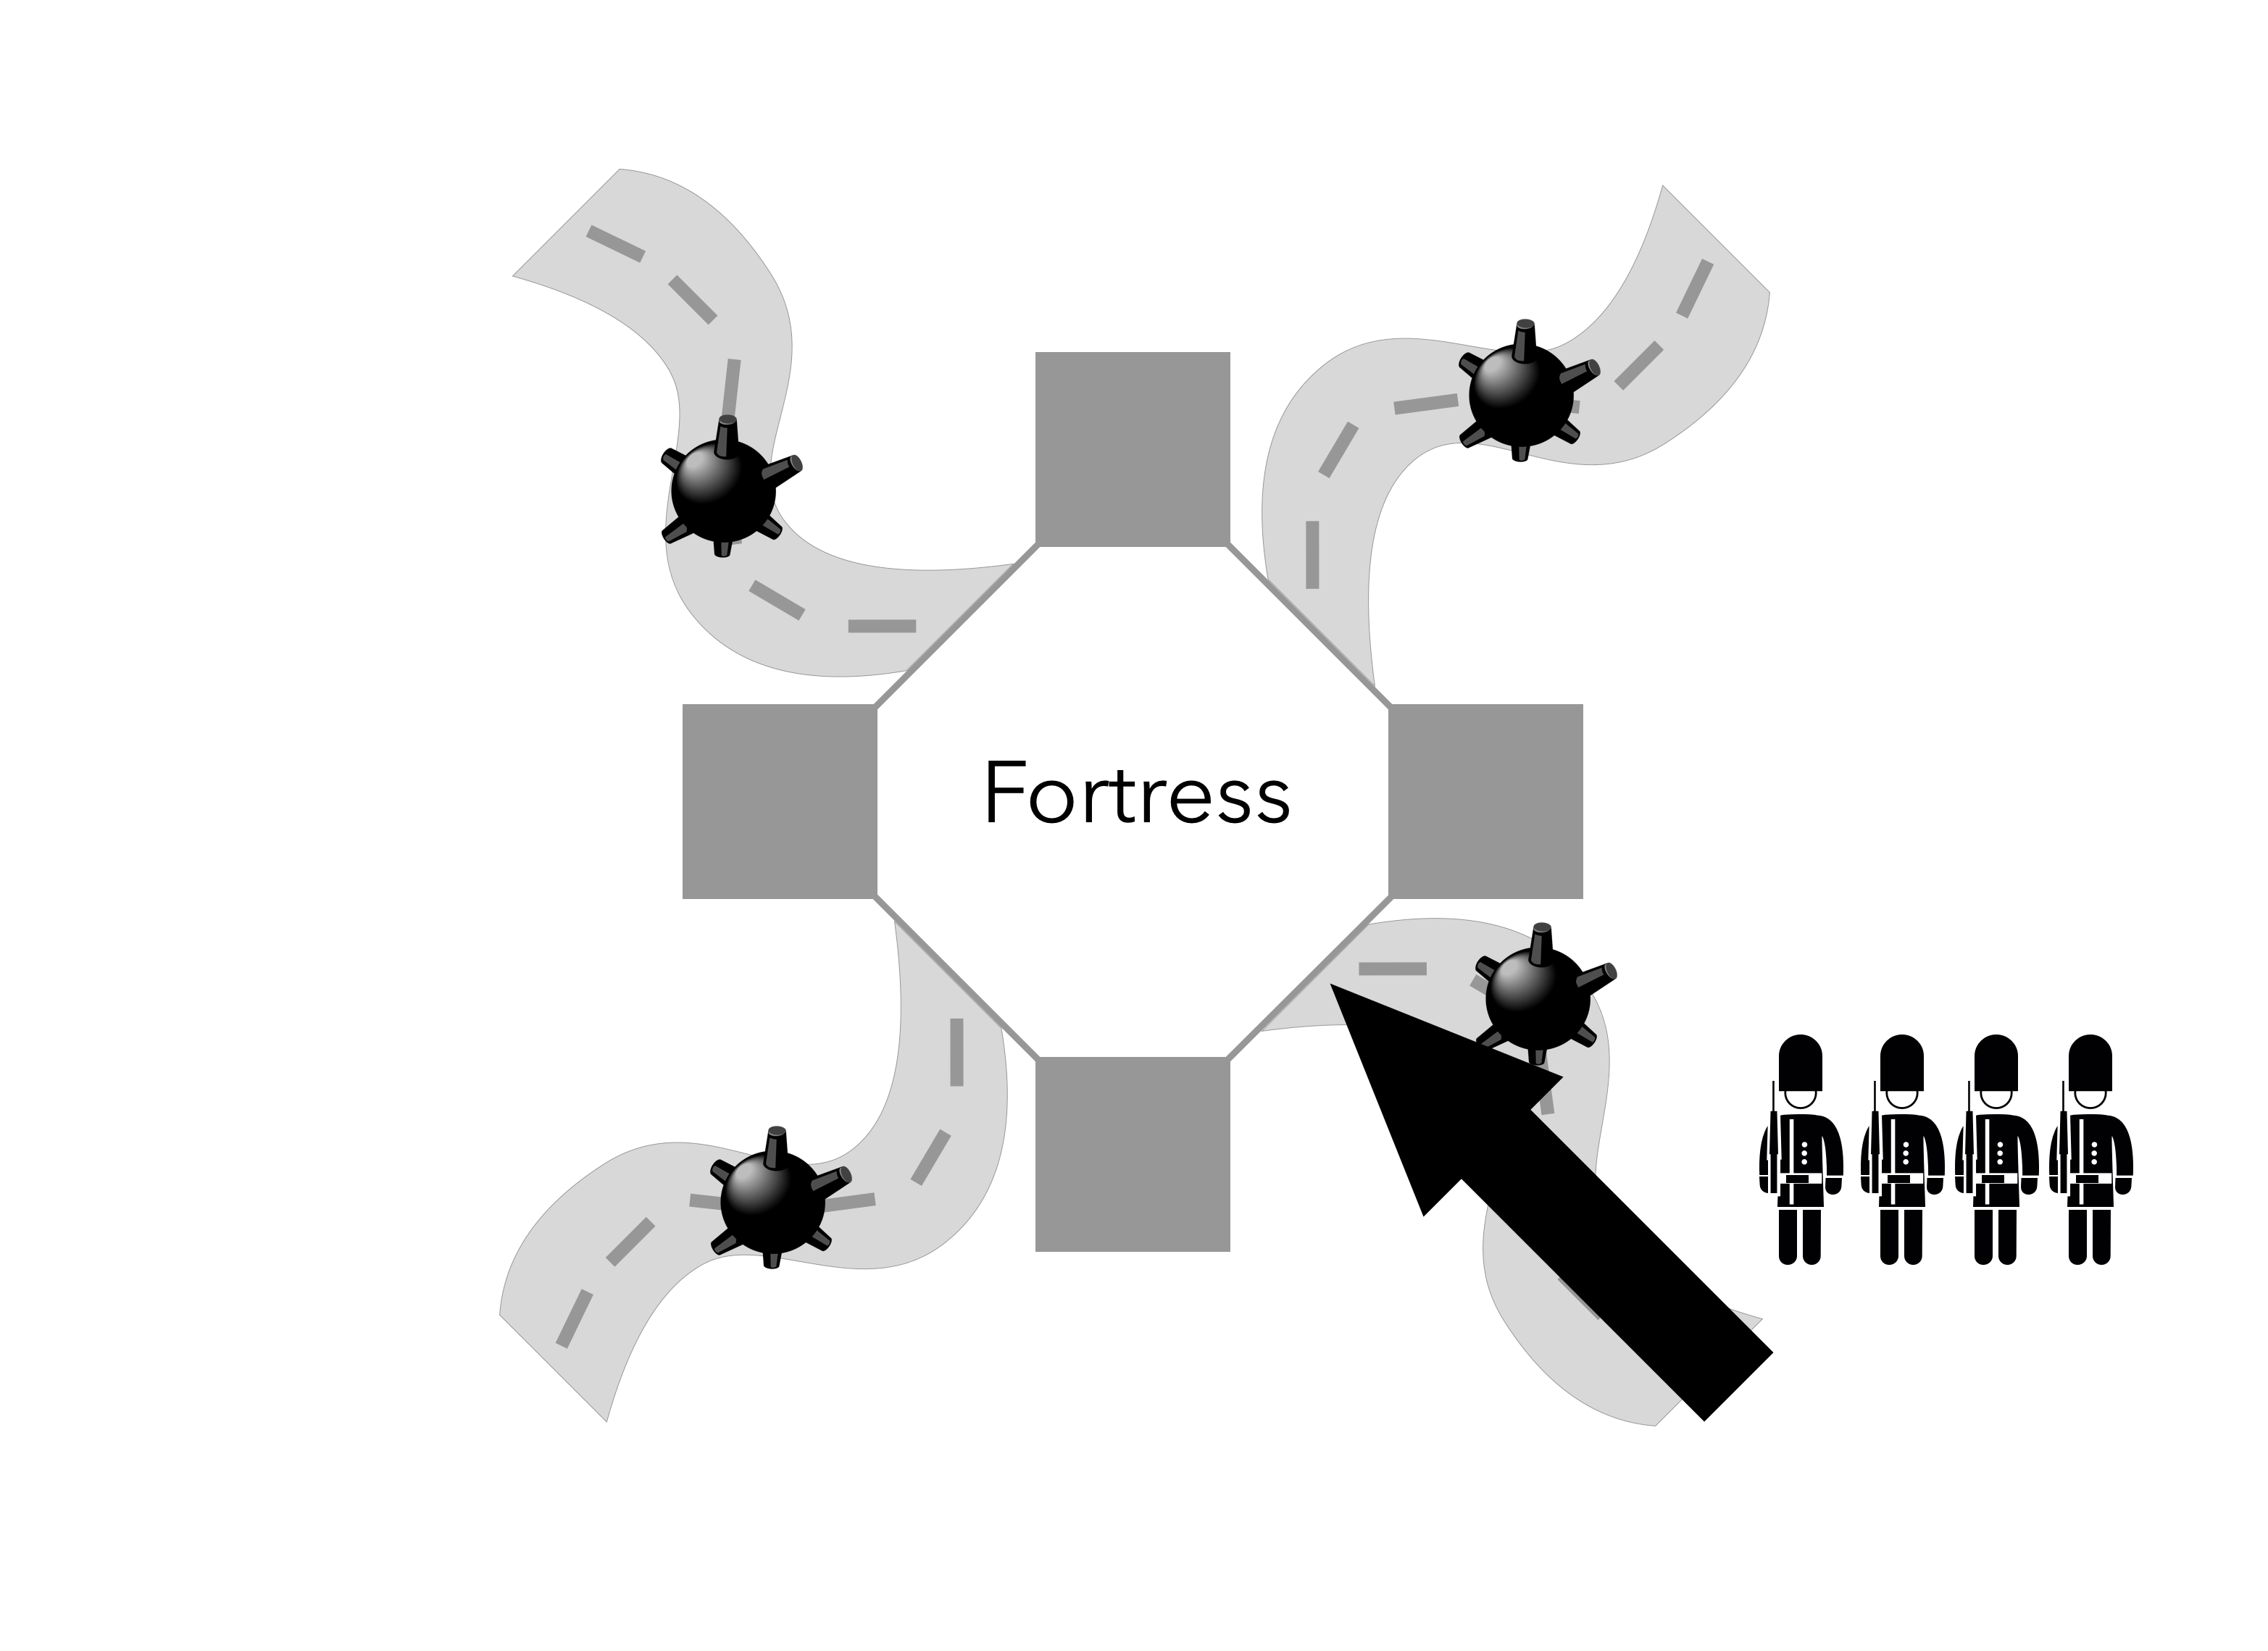
\includegraphics[scale=0.07]{images/fortress_problem.png}
    	\caption{Initial situation of the fortress problem}
    	\centering
    	\label{fig:fortress}
    \end{minipage}
    \hfill
    \begin{minipage}[b]{0.40\textwidth}
    	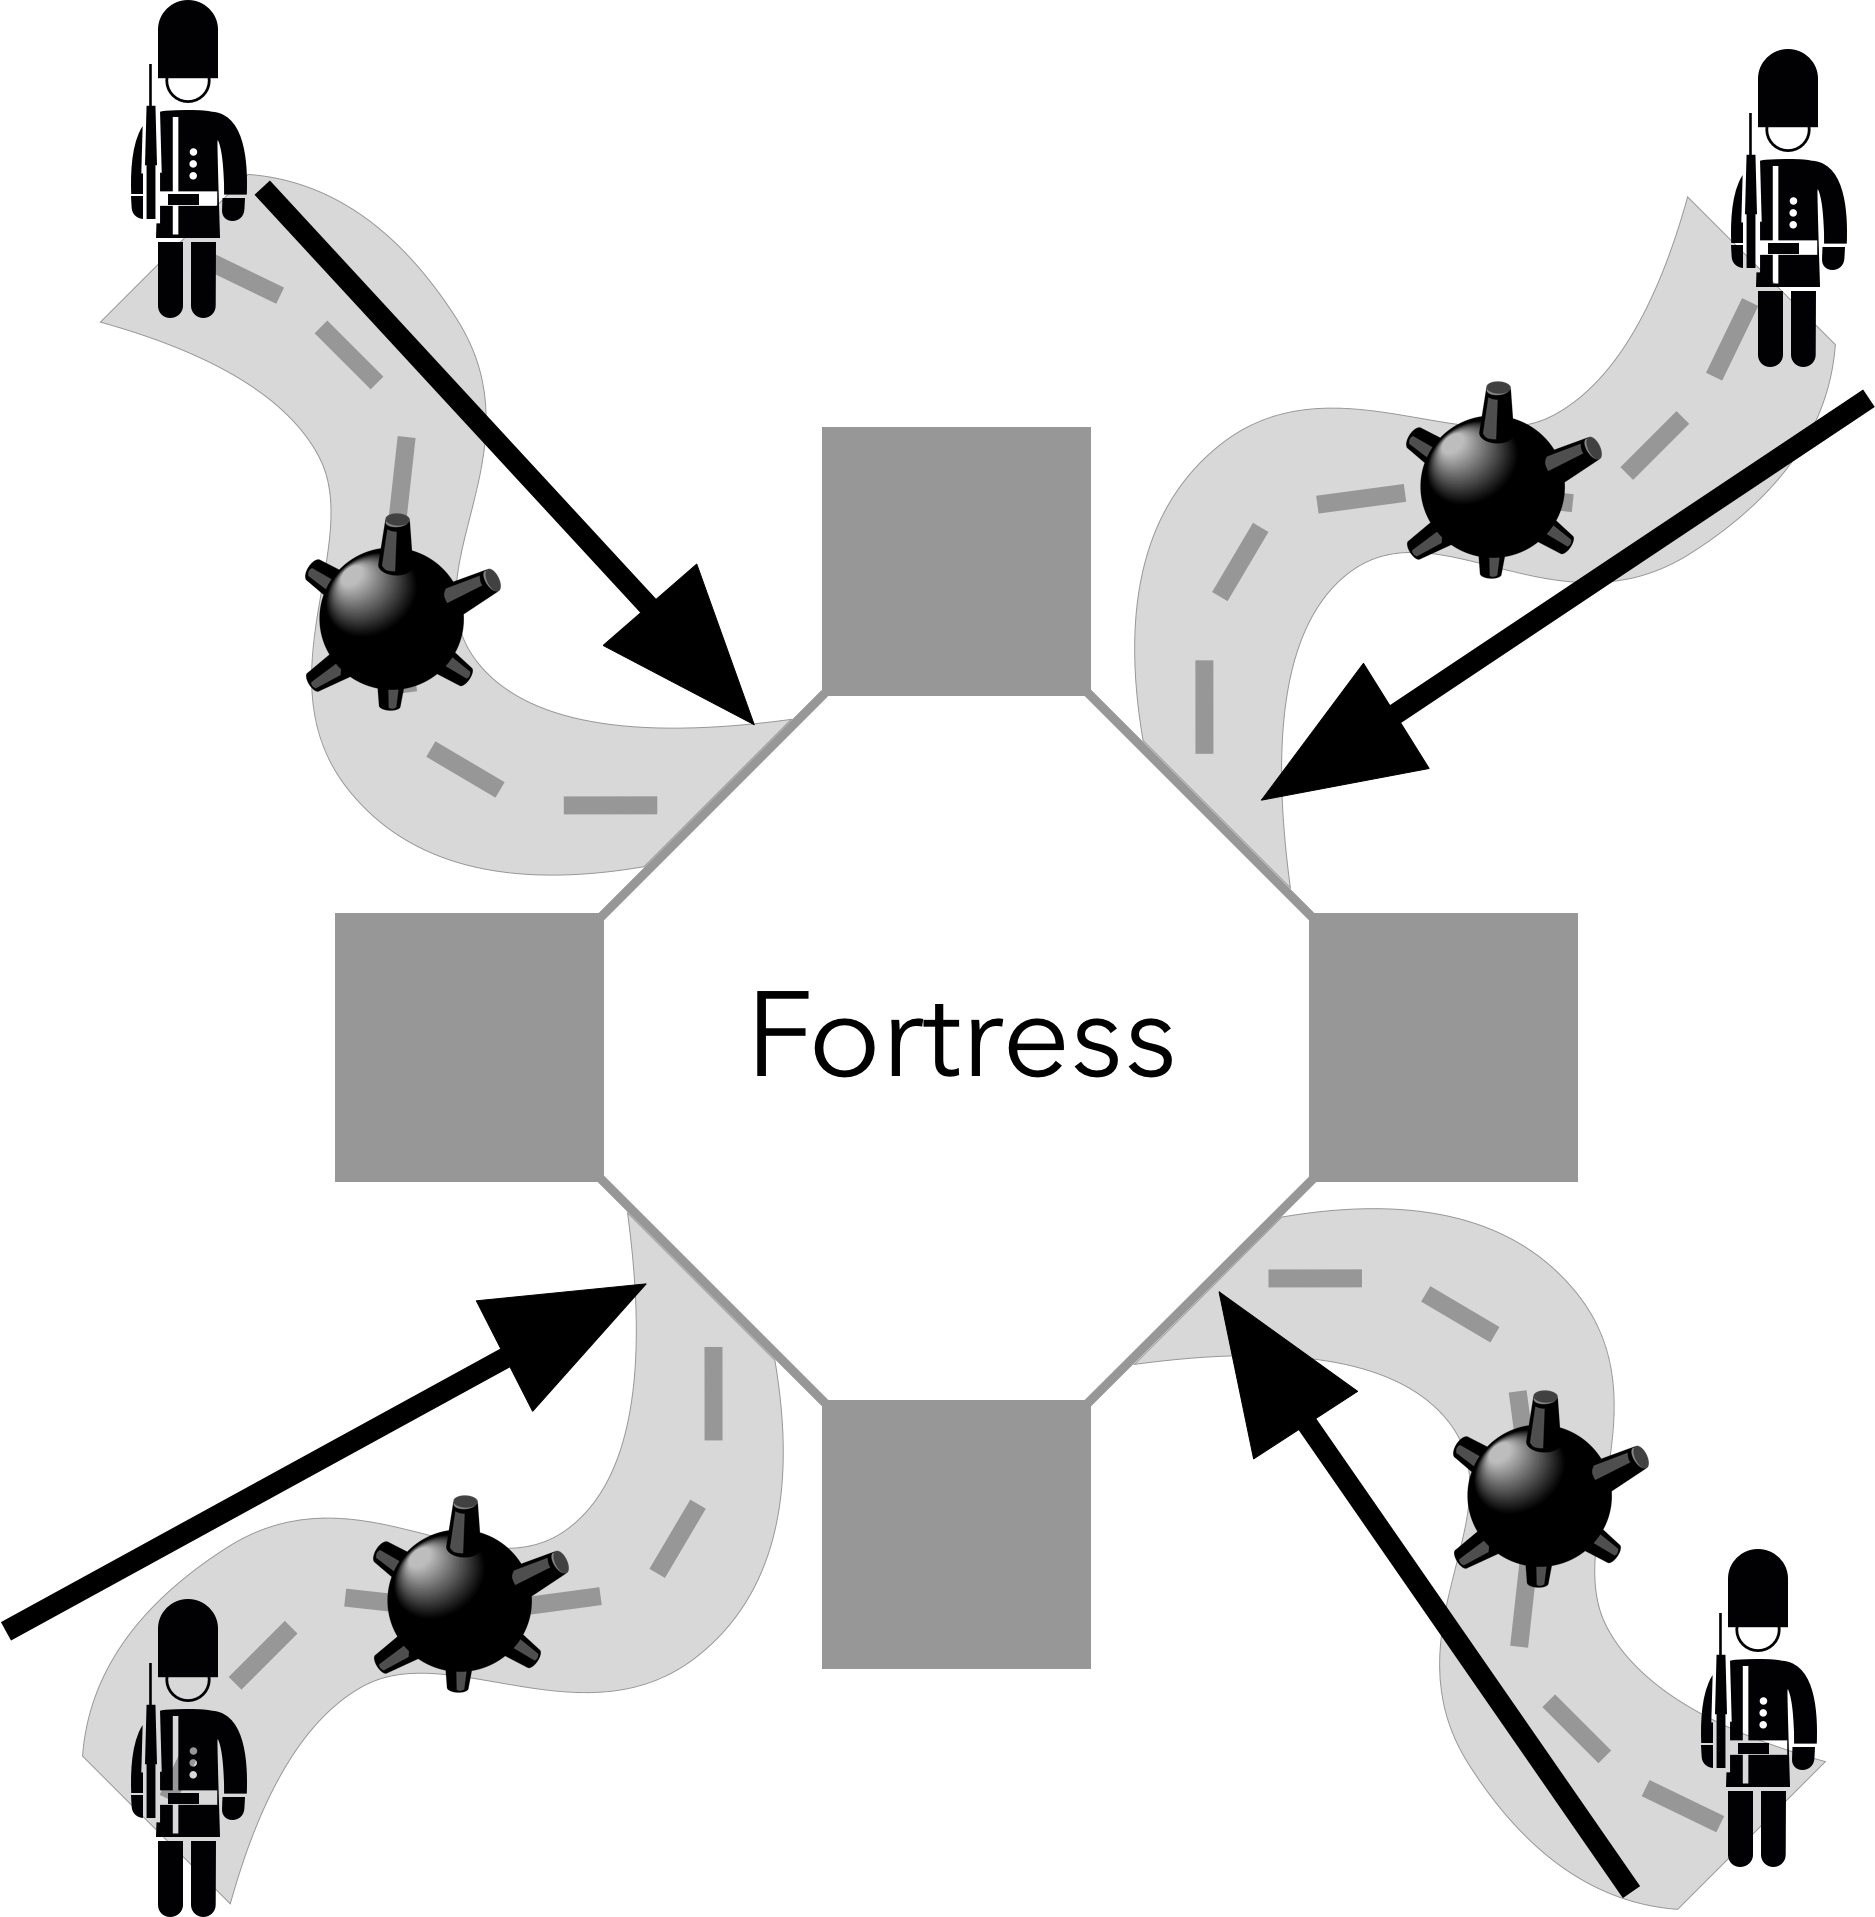
\includegraphics[scale=0.07]{images/fortress_problem_solution.png}
    	\caption{Solution for the fortress problem}
    	\centering
    	\label{fig:fortress_solution}
    \end{minipage}
\end{figure}

Now they get a new different problem as stated as from Gick and Holyoak \cite[307-308]{gick1980analogical}: "Suppose you are a doctor faced with a patient who has a malignant tumour in his stomach. It is impossible to operate on the patient, but unless the tumour is destroyed the patient will die. There is a kind of ray that can be used to destroy the tumour. If  the rays reach the tumour all at once at a sufficiently high intensity, the tumour will be destroyed. Unfortunately, at this intensity the healthy tissue that the rays pass through on the way to the tumour will also be destroyed. At lower intensities the rays are harmless to healthy tissue, but they will not affect the tumour either. What type of procedure might be used to destroy the tumour with the rays, and at the same time avoid destroying the healthy tissue?". Finally, the participants are asked to solve the tumour problem. The expected behaviour is now that the participants are able to find a solution by looking at the sketch and use an analogy they've learned from the fortress problem before. Figure \ref{fig:radiation_problem} illustrates again the initial scenario and figure \ref{fig:radiation_solution} the solution.

\begin{figure}[H]
    \centering
    \begin{minipage}[b]{0.45\textwidth}
    	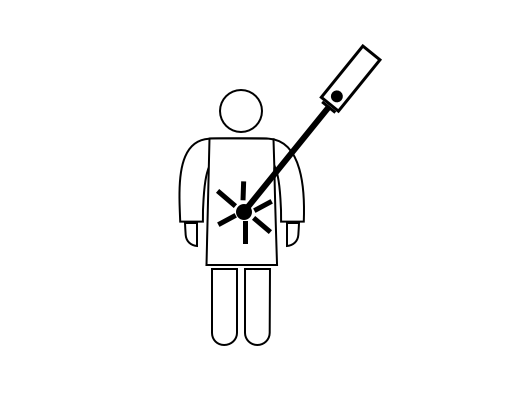
\includegraphics[scale=0.3]{images/laser_1.png}
    	\centering
    	\caption{Initial situation of the radiation problem}
    	\label{fig:radiation_problem}
    \end{minipage}
    \hfill
    \begin{minipage}[b]{0.45\textwidth}
    	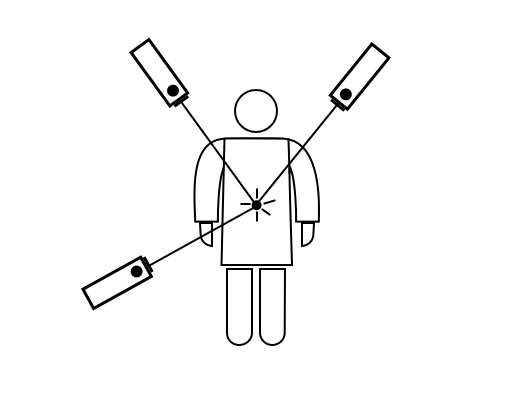
\includegraphics[scale=0.3]{images/laser_2.png}
    	\centering
    	\caption{Solution for the radiation problem}
    	\label{fig:radiation_solution}
    \end{minipage}
\end{figure}


% Hier noch die Lösung für das Radiation Problem nieder schreiben, also das 3 Laser zusammen eintreffe.
\newpage
As you can see in the solution, the large (powerful) laser, which is an analogy to the army, is divided into several smaller (less powerful) lasers. By irradiation from several directions, which is then bundled in the tumour, it is possible to destroy it without the laser emitting a harmful amount of radiation to the patient. 
Even though using this analogy was not obvious enough for the participants in the study of Gick and Holyoak as subjects had to explicitly get told that the military problem would be applicable to successfully solve the radiation problem, it should already give a better idea of how we might draw a solutions by using the source design case to the target problem. A major difference to all the case studies that were performed on this topic before and this one is, that this paper hypothesizes that at least in design, humans can usefully represent the problem-solving procedures using visuospatial representations in which relation between cause, impact and intent is mostly implicit. The following chapter will focus on the detailed research described and analysed based on a cognitive study conducted by Craig \cite{craig2001perceptual} on novice designers and it's respective results. The chapter will also describe the computer program (Galatea) they were using to simulate visuospatial in- and output representations of some of the participants that took part of the study. Closing with a discussion on the findings and a brief evaluation of the results. 
\section{Overview of Research} %Research Goal noch mal erwähnen, also dass wir über Design Analogien vertehen, das fehlt noch
Basis of the analysis performed was Craig's \cite{craig2001perceptual} %noch mal nachschauen
data that he captured in his doctoral publication about 34 novice designers from the Georgia Institute of Technologies. In this study 34 undergraduate students were shown a source design case about a clean room laboratory. 
This source design case contained a description of a design problem in a written form of text and a corresponding drawing of the solution for the given problem. Right afterwards the participants of the study were encouraged to solve an analogous design problem. This time the problem was represented with text only and it was up to the participants to draw a solution based on the solution of the first design case. %text von Freitag
The problem initially presented to the study participants deals with a scenario in which a computer chip manufacturer has to be very meticulous in ensuring that the environment within the chip manufacturing laboratory is as sterile as possible. The laboratory is a closed area with a gate that is the only way to get into the room. The highest goal is therefore to keep the environment in the laboratory sterile, dust-free and without unwanted gases. The gate is the weak point in the whole construction because every time an employee enters the laboratory, the seal (the gate) is broken or opened and dirt can enter. The company is now trying to develop a new door that allows employees to enter and leave the laboratory easily and uncomplicated, while mitigating the problem of contamination as much as possible. The solution to the problem follows the textual description of the problem by the computer chip manufacturer, in this case in the form of a sketch. The solution involves creating a form of intermediate area from the original gate and placing this area in front of the laboratory. This area can be imagined as a kind of pressure chamber, i.e. we have a sealed room with a door on both sides. One side of the opening faces the dirty outside world, the other side the clean laboratory. When the employee enters the gap through the outside world, he does not bring the dirt into the room into the laboratory. The door closes and the employee who is now in the room closed on both sides can be freed from all impurities (e.g. by showers or ventilation systems that suck the dirty air away). The chamber is now cleaned and the employee can enter the laboratory through the second door without risk. In summary, the concept is that employees enter a chamber with two doors. Figure \ref{fig:input_conditions} displays the solution concept that was presented to the students in two different forms of visualizations named \textit{condition 1} and \textit{condition 2}.

\begin{figure}[H]
  \centering
  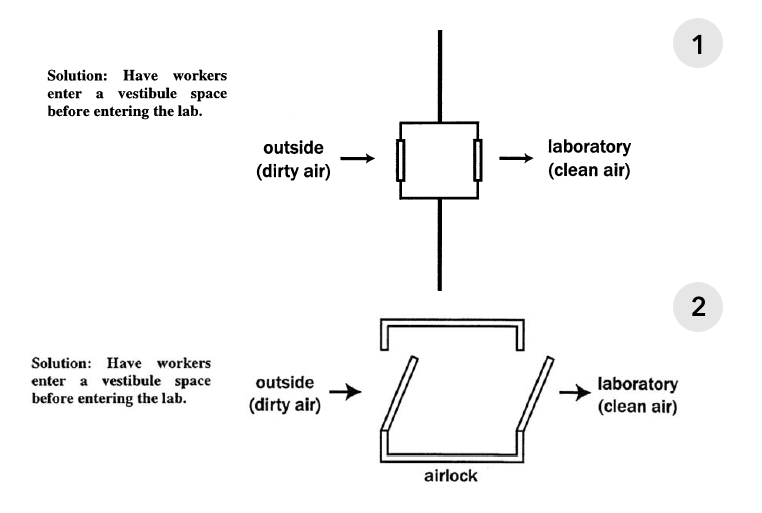
\includegraphics[width=0.7\linewidth]{images/input_conditons.PNG}
  \caption{\label{fig:input_conditions} Condition 1 and Condition 2 \\ Top view of lab, with the vestibule.}
\end{figure}     

After the study participants have studied the first problem description and problem sketch, the second problem is presented to them in the form of a text. 
The second text is that the Ministry of Transport has designed a vehicle to cut grass at the roadside. For this purpose a long rod was attached to the side of the vehicle, at the end of which a kind of lawn mower was fixed. This enables the vehicle to drive along the roadside and at the same time remove the edges of the road from high grass. The problem here, however, is that it regularly happens that mailbox posts, lanterns or telephone poles get in the way and block the arm with the cutting mechanism. Since the posts are too high, it is not an option to simply lift the cutting arm over the blockade. Pulling in or folding away the cutting arm is also not an option as this would severely disrupt the grass cutting process. Therefore the Road Traffic Department tries to design a pole that can pass through the masts and posts without interrupting the cutting process. The solution to this problem is now to be provided by the study participants, taking into account the solution from the first case. In doing so, they should take into account every idea, however small, and record their approach to solving the problem as sketched.  From the 34 participants 15 of them were able to create an adequate solution according to the requirements of the 2nd case. 

\begin{figure}[h!]
  \centering
    \begin{subfigure}[b]{0.8\linewidth}
    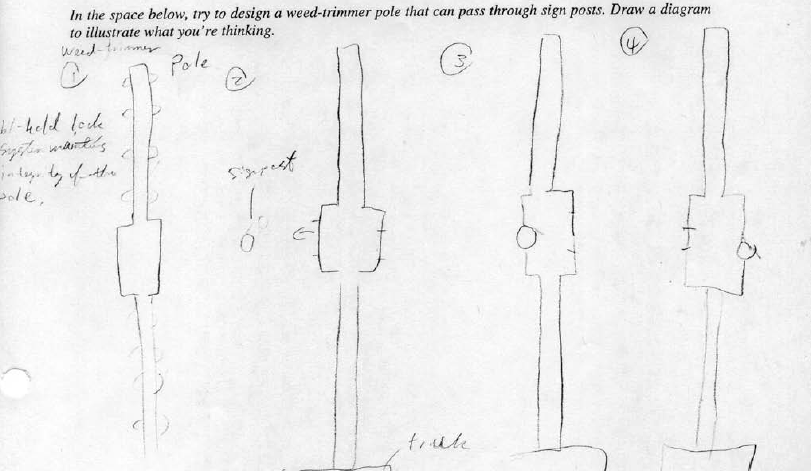
\includegraphics[width=\linewidth]{images/drawing_l24_con2.PNG}
    \caption{Participant L24`s solution received condition 2 (Fig. \ref{fig:input_conditions})}
  \end{subfigure}
  \begin{subfigure}[b]{0.3\linewidth}
    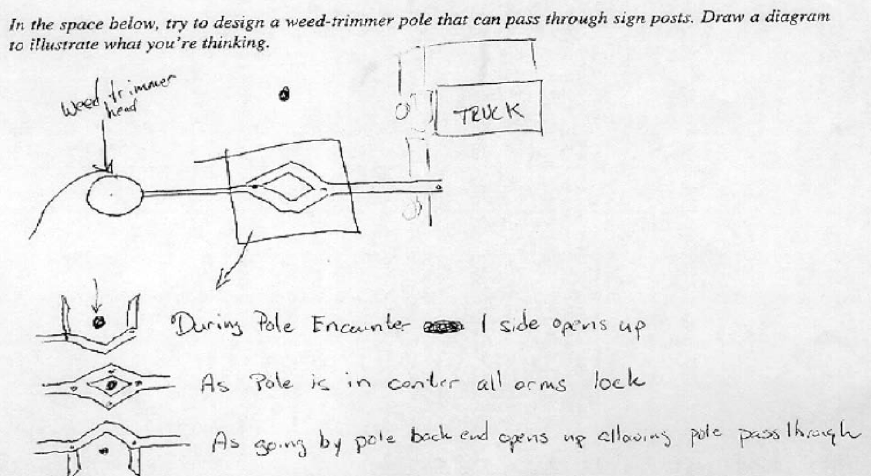
\includegraphics[width=\linewidth]{images/drawing_l15_con2.PNG}
     \caption{Participant L15}
  \end{subfigure}
  \begin{subfigure}[b]{0.3\linewidth}
    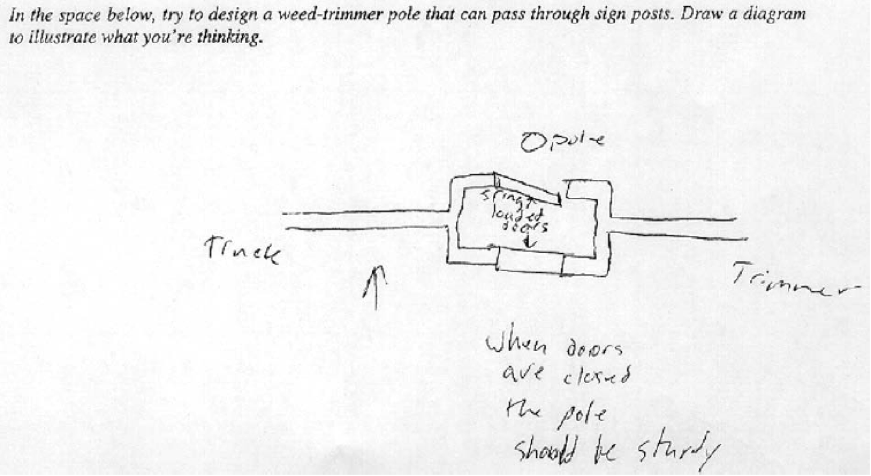
\includegraphics[width=\linewidth]{images/drawing_l16_con1.PNG}
    \caption{Participant L16}
  \end{subfigure}
  \begin{subfigure}[b]{0.3\linewidth}
    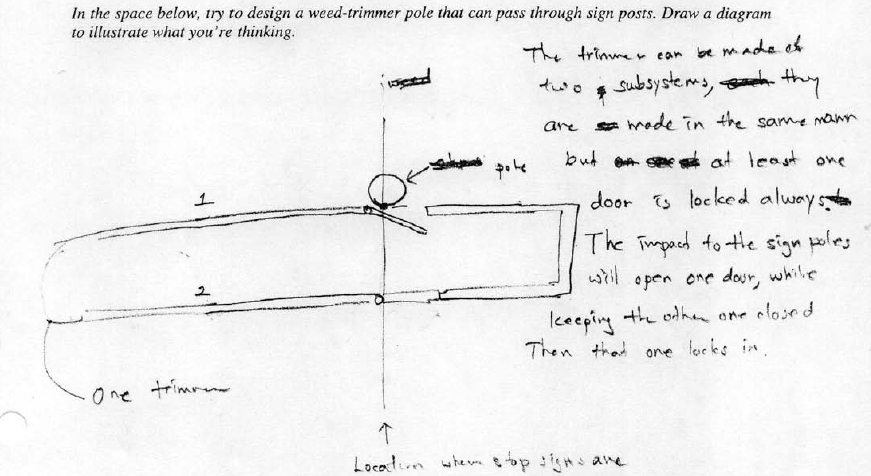
\includegraphics[width=\linewidth]{images/drawing_l22_con2.PNG}
    \caption{Participant L22}
  \end{subfigure}
  \caption{An extract of the some correct sketches created by the participants}
  \label{fig:drawing_l24_con2}
\end{figure}

The correct solution for this problem has been to design a bar containing two locking doors in the cutting post as the correct solutions of the participants in Figure \ref{fig:drawing_l24_con2} demonstrate. The lantern poles and telephone poles can now (analogous to the solution in the first case) be inserted into the pole via one door and out again via the second door on the other side via the two doors. Of course, such a solution requires that while one side of the cutter bar is open, the other side ensures that the device remains stable and vice versa. The concept of the solution therefore remains the same as in the previous scenario. It should also be noted that each of the 34 participants was presented with a version of two different initial versions. These versions differed slightly in the wording of the text and the solution to the first case was sketched slightly differently. In terms of content, however, both were identical. In the sketches of the 15 participants who were able to solve the problem correctly, many differences could be found in their editions. Figure \ref{fig:summary_differences} shows a table of all spotted differences in the drawings. 

\begin{figure}[H]
  \centering
  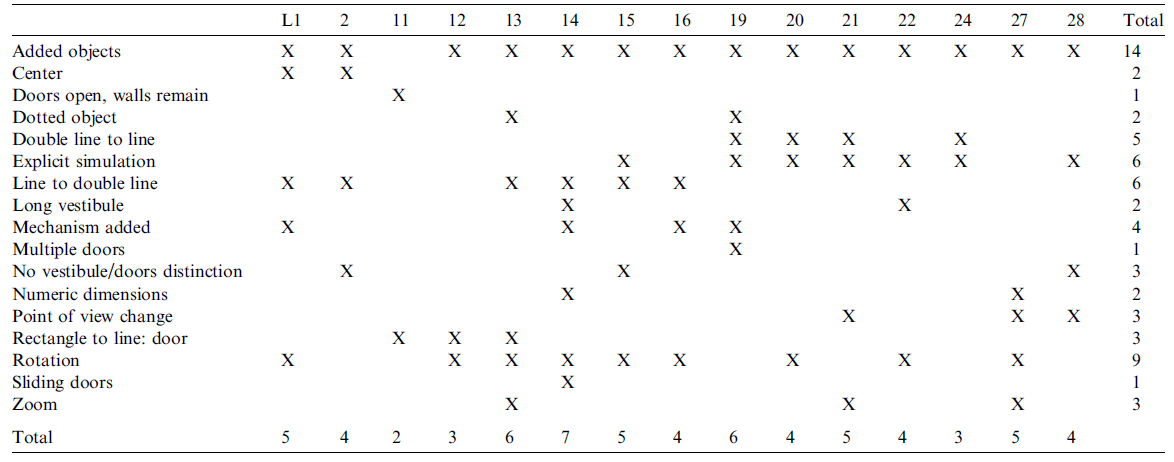
\includegraphics[width=\linewidth]{images/table_differences_of_solutions.PNG}
  \caption{\label{fig:summary_differences}Observed differences in the drawings of the 15 participants. Type of the difference are shown on the Y axis, participant number on the X axis.
}
  
\end{figure}     

It could be observed that all participants who were able to transfer the analogy from the first case into their drawings were also able to find the correct solution to the problem. For the 14 participants who could not provide a solution, it is assumed that they understood the analogy but were not able to figure out how to use it effectively or simply ignored the hint to use the analogy. Based on the students' correctly produced drawings, 4 solutions were transferred using Galatea, a software program for modeling visual knowledge. Galatea allows multi-level problem-solving procedures to be represented as a set of states of knowledge and transformation between states. The elements of each state of knowledge are instances of visual elements, and the operations are visual transformations.  States of knowledge consist of visual knowledge represented symbolically, the so-called \textit{s-images} (symbolic images). 
The other 10 were transferred using pen and paper models. All the models, whether transferred using Galatea or pen and paper, are implemented based on a theory from Jim Davies' dissertation \textit{Constructive Adaptive Visual Analogy} \cite{davies2004constructive}. This theory claims that visual knowledge is helpful in solving problems analogously and suggests a mechanism for achieving it. The same mechanism, in conjunction with the modelling language Covlan\footnote{Covlan is a visual knowledge representation language for representing visual knowledge and supporting visual reasoning \cite{davies2007transfer}}, which allows structures and internal processes to be defined at a higher level of abstraction, is here used for the mapping of the participants drawings to models. To enable this for Galatea being able to make this analogical transfer it is necessary that the source and target analogues must have an analogy between them. Its algorithm processes the set of input \textit{s-images} of the source case and the targets by identifying the corresponding two starter \textit{s-images}. Then it identifies the transformation made with their associated arguments in the current \textit{s-image} of the source case to find out how the source case gets from the current \textit{s-image} state to the next one. Then it identifies the objects of the transformations. The object of the transformation is what object, the transformation acts on. Now as the fourth step Galatea tries to find the corresponding objects in the target problem and will as the next step map the transformation with its arguments to target \textit{s-image}. Then it maps the original objects in the target to the new objects in the target and following it then maps the new objects of the target case to the corresponding objects in the source case. Finally it is checked if there are more s-images, should this be the case then the process is finished and the solution is transferred. If there are more s-images in the source case, the whole process will start at the beginning again and the system will try to identify the current source and target s-images and so on. In order to be able to evaluate the 15 models, the authors investigated how well the models take into account the differences between the source sketch and the participant sketch. It should be noted that the solution sketch from the first case is very strongly derived from the actual image of the laboratory. It is so far derived, that the functionality which results from the sketch could have been transferred one-to-one to the solution of the cutting arm without changing the solution sketch. Later in this essay, it will be shown that each participant has deviated slightly from the source solution. These distinctions between the participant's sketch and the solution sketch indicate the differences between the participants. In order to be able to continue with the modelling according to Craig's theory, it was necessary to determine the Covlan representation for the source sketch and, as already mentioned, the participants' drawings of the  \textit{s-images} to further process it to be able to create model out of them. 

\begin{figure}[H]
  \centering
  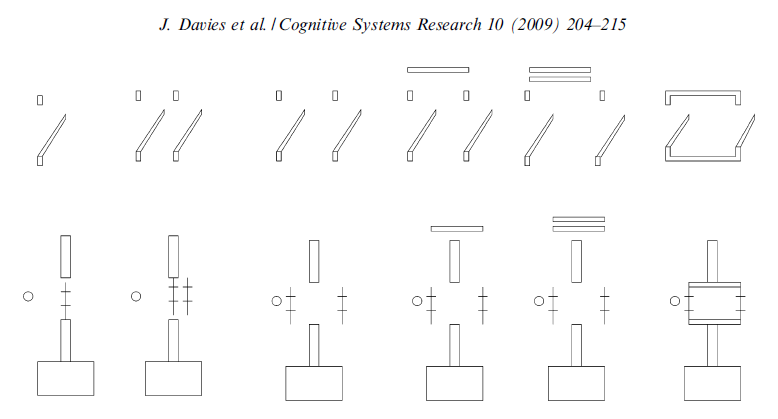
\includegraphics[width=0.7\linewidth]{images/covlan_L24.PNG}
  \caption{\label{fig:covlan_l24}\textit{s-images} of the source solution (top row) and the solution of participant L24 (bottom row)}
\end{figure}  

Using the hypothesis of the researchers that a visual-spatial representation of states of knowledge, organized in chronological order, can enable the transfer of problem-solving procedures, the participants' outputs are predicted. And thus to evaluate the models created, the predicted output was compared with differences from the participants' data. What you can see in figure \ref{fig:covlan_l24} is the model of the participant L24. Each row represents a series of s-images. The upper row shows the series of s-images according to Galateas its representation for the source solution (the vestibule space in front of the laboratory) and the lower row the representation of the model for the participant L24. Each single s-image in the respective rows represents a further transformation that was performed necessary to reach the final picture. With reference to the first series, the researchers assume that this shows the steps necessary to achieve the source solution. It is assumed that this transformation is done mentally by the participants when they look at the source solution through the two-dimensional image and text that we could see in Figure \ref{fig:input_conditions}. The second series is L24's transformation from the source problem to the correct solution. If you look at the first \textit{s-image} on the lower left side of fig. \ref{fig:covlan_l24}, you can see the start state of the grass-cut vehicle. The large square represents the car, the circle represents a mast and the right-angled cutting arm. What happens now is the step-by-step transformation from the source problem to the target problem. This consists of 5 parts. The first one involves duplicating the door elements, taking a set necessary to form a door and duplicating it. As a second step, in relation to the dimensions of the door, the newly created doors are brought into the correct position. The third and fourth step involves adding new components (top and bottom walls) to complete the chamber. In the 5 and final step, the correct relationship of the individual parts is made, and the double door system is completed. Of fundamental importance for the statement made in the researchers' paper is the mapping of the respective states in the s-images to be seen in Figure 6. A comparison of the upper row with the lower row shows that the individual transformations have been transferred to the new problem. For example, the second s-image of the lower row shows, as in the second s-image of the first row, that objects have been replicated.
Furthermore, the researchers were able to predict the analogue thinking of participant L24 with their model. The performed transformations maintained the change from double lines (the double line walls in Condition 2 in Fig. \ref{fig:input_conditions}) to single and adding further elements.  If we now look again at the drawing of L24 (see Fig. \ref{fig:drawing_l24_con2}a ) it can be seen that the participant had extended his construction with the help of a small picture by picture explanation in which it becomes clear how the lantern pole is led through the cutting rod.  However, the researchers were unable to describe this simulation using Covlan, as this tool is intended for describing diagram-like inscriptions and not for mapping mental models. Overall, it can be said that the model for L24 contains two out of three found differences: the double line to single line transformation and the addition of objects, but not the explicit simulation.

\begin{figure}[H]
  \centering
  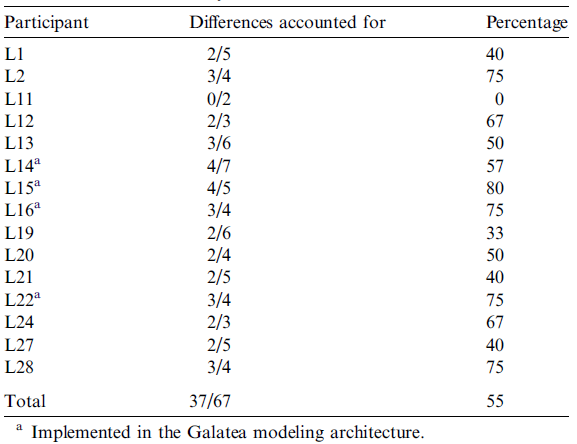
\includegraphics[width=0.7\linewidth]{images/differences_found.PNG}
  \caption{\label{fig:differences_found}Differences accounted for by Galatea modelling}
\end{figure}  

%\begin{wrapfigure}{r}{0.5\textwidth}
%  \begin{center}
%  	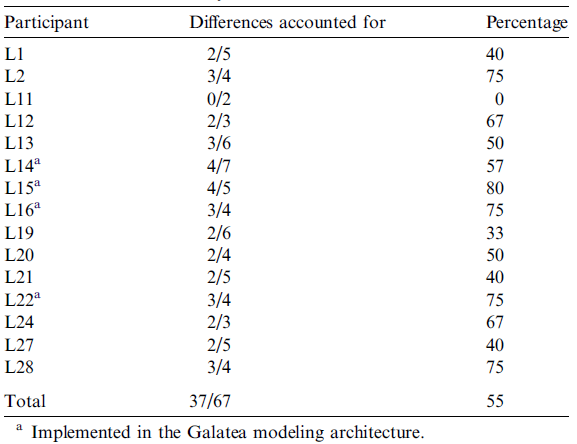
\includegraphics[width=0.7\linewidth]{images/differences_found.PNG}
%  	\caption{\label{fig:differences_found}}
%  \end{center}
%  \caption{A gull}
%\end{wrapfigure}


Models were also created for the other 14 participants who were able to create a correct solution. The models of the participants L14, L15, L15 and L22 were implemented with Galatea, the remaining models were created with pen and paper taking Galatea's representation and processing into account. The Figure \ref{fig:differences_found} shows for how many of the differences made by the participant the model was successful in accounting these differences. In total, slightly more than half of the differences could have been accounted using the researchers' models. This is to show how using pure visual representation it is possible to create design drawings only on the basis of analogies because the models were able to locate many of the differences made by the participants. The researchers demonstrate that designers are able to create new structures and constructs if they are introduced to the topic of design-by-analogy and explicitly encouraged to take this approach. By looking at problem solutions visually we enable them to extract essential properties that have contributed to the solution of the problem. These properties, in turn, can be mapped to a new problem by a visual-spatial presentation of the participants and thus make an essential contribution to finding the solution. Thus the authors demonstrate how purely spatial-visual knowledge is used to solve problems. 



\section{Discussion / Critical Evaluation}



%Please discuss the research you reviewed in the above section. For instance,
%\begin{itemize}
%\item What's good about it?
%\item What has been achieved?
%\item To what extent does it live up to its aspirations?
%\item Take up concerns / comments mentioned during corresponding seminar sessions.
%\item How is this research related to other aspects / topics treated in the scope of the seminar?
%\end{itemize}

\noindent

\bibliographystyle{apacite}

\bibliography{bib}

\end{document}